%\chapter*{Неделя 12}
\protect\thispagestyle{fancy}
\section{}
Пусть выходные отсчёты нерекурсивного фильтра 1-ого порядка получаются усреднением текущего и предшествующего входных отсчётов
\begin{equation*}
	y[k] = 0.5x[k] + 0.5x[k-1].
\end{equation*}

Найти импульсную характеристику $h[k]$ и переходную характеристику фильтра $g[k]$, определить время установления по переходной характеристике. Построить нуль-полюсную диаграмму и исследовать фильтр на устойчивость.

\begin{equation*}
	\Capit{H}(z) = \dfrac{\Capit{Y}(z)}{\Capit{X}(z)} = 0.5 (1 + z^{-1}) = h[0] + h[1]z^{-1}, \quad \Rightarrow h[k] = 
	\begin{cases}
		0.5, & \text{если } k = 0 \text{ или } k=1,\\
		0, & \text{иначе}.
	\end{cases}
\end{equation*}

\begin{equation*}
	g[k] = \sum \limits_{m = 0}^{+\infty} h[k + m] = 
	\begin{cases}
		0.5, & \text{если } k = 0,\\
		1, & \text{если } k \geq 1,\\
		0, & \text{иначе}.
	\end{cases}
\end{equation*}

Время установления -- $1$ такт (если считать с нулевого).

\begin{equation*}
	\Capit{H}(z) = 0.5 (1 + z^{-1}) = \dfrac{1 + z}{2z},\quad \Rightarrow
	z_{p} = 0, z_{o} = -1.
\end{equation*}

\begin{figure}[!h]
	\centering
	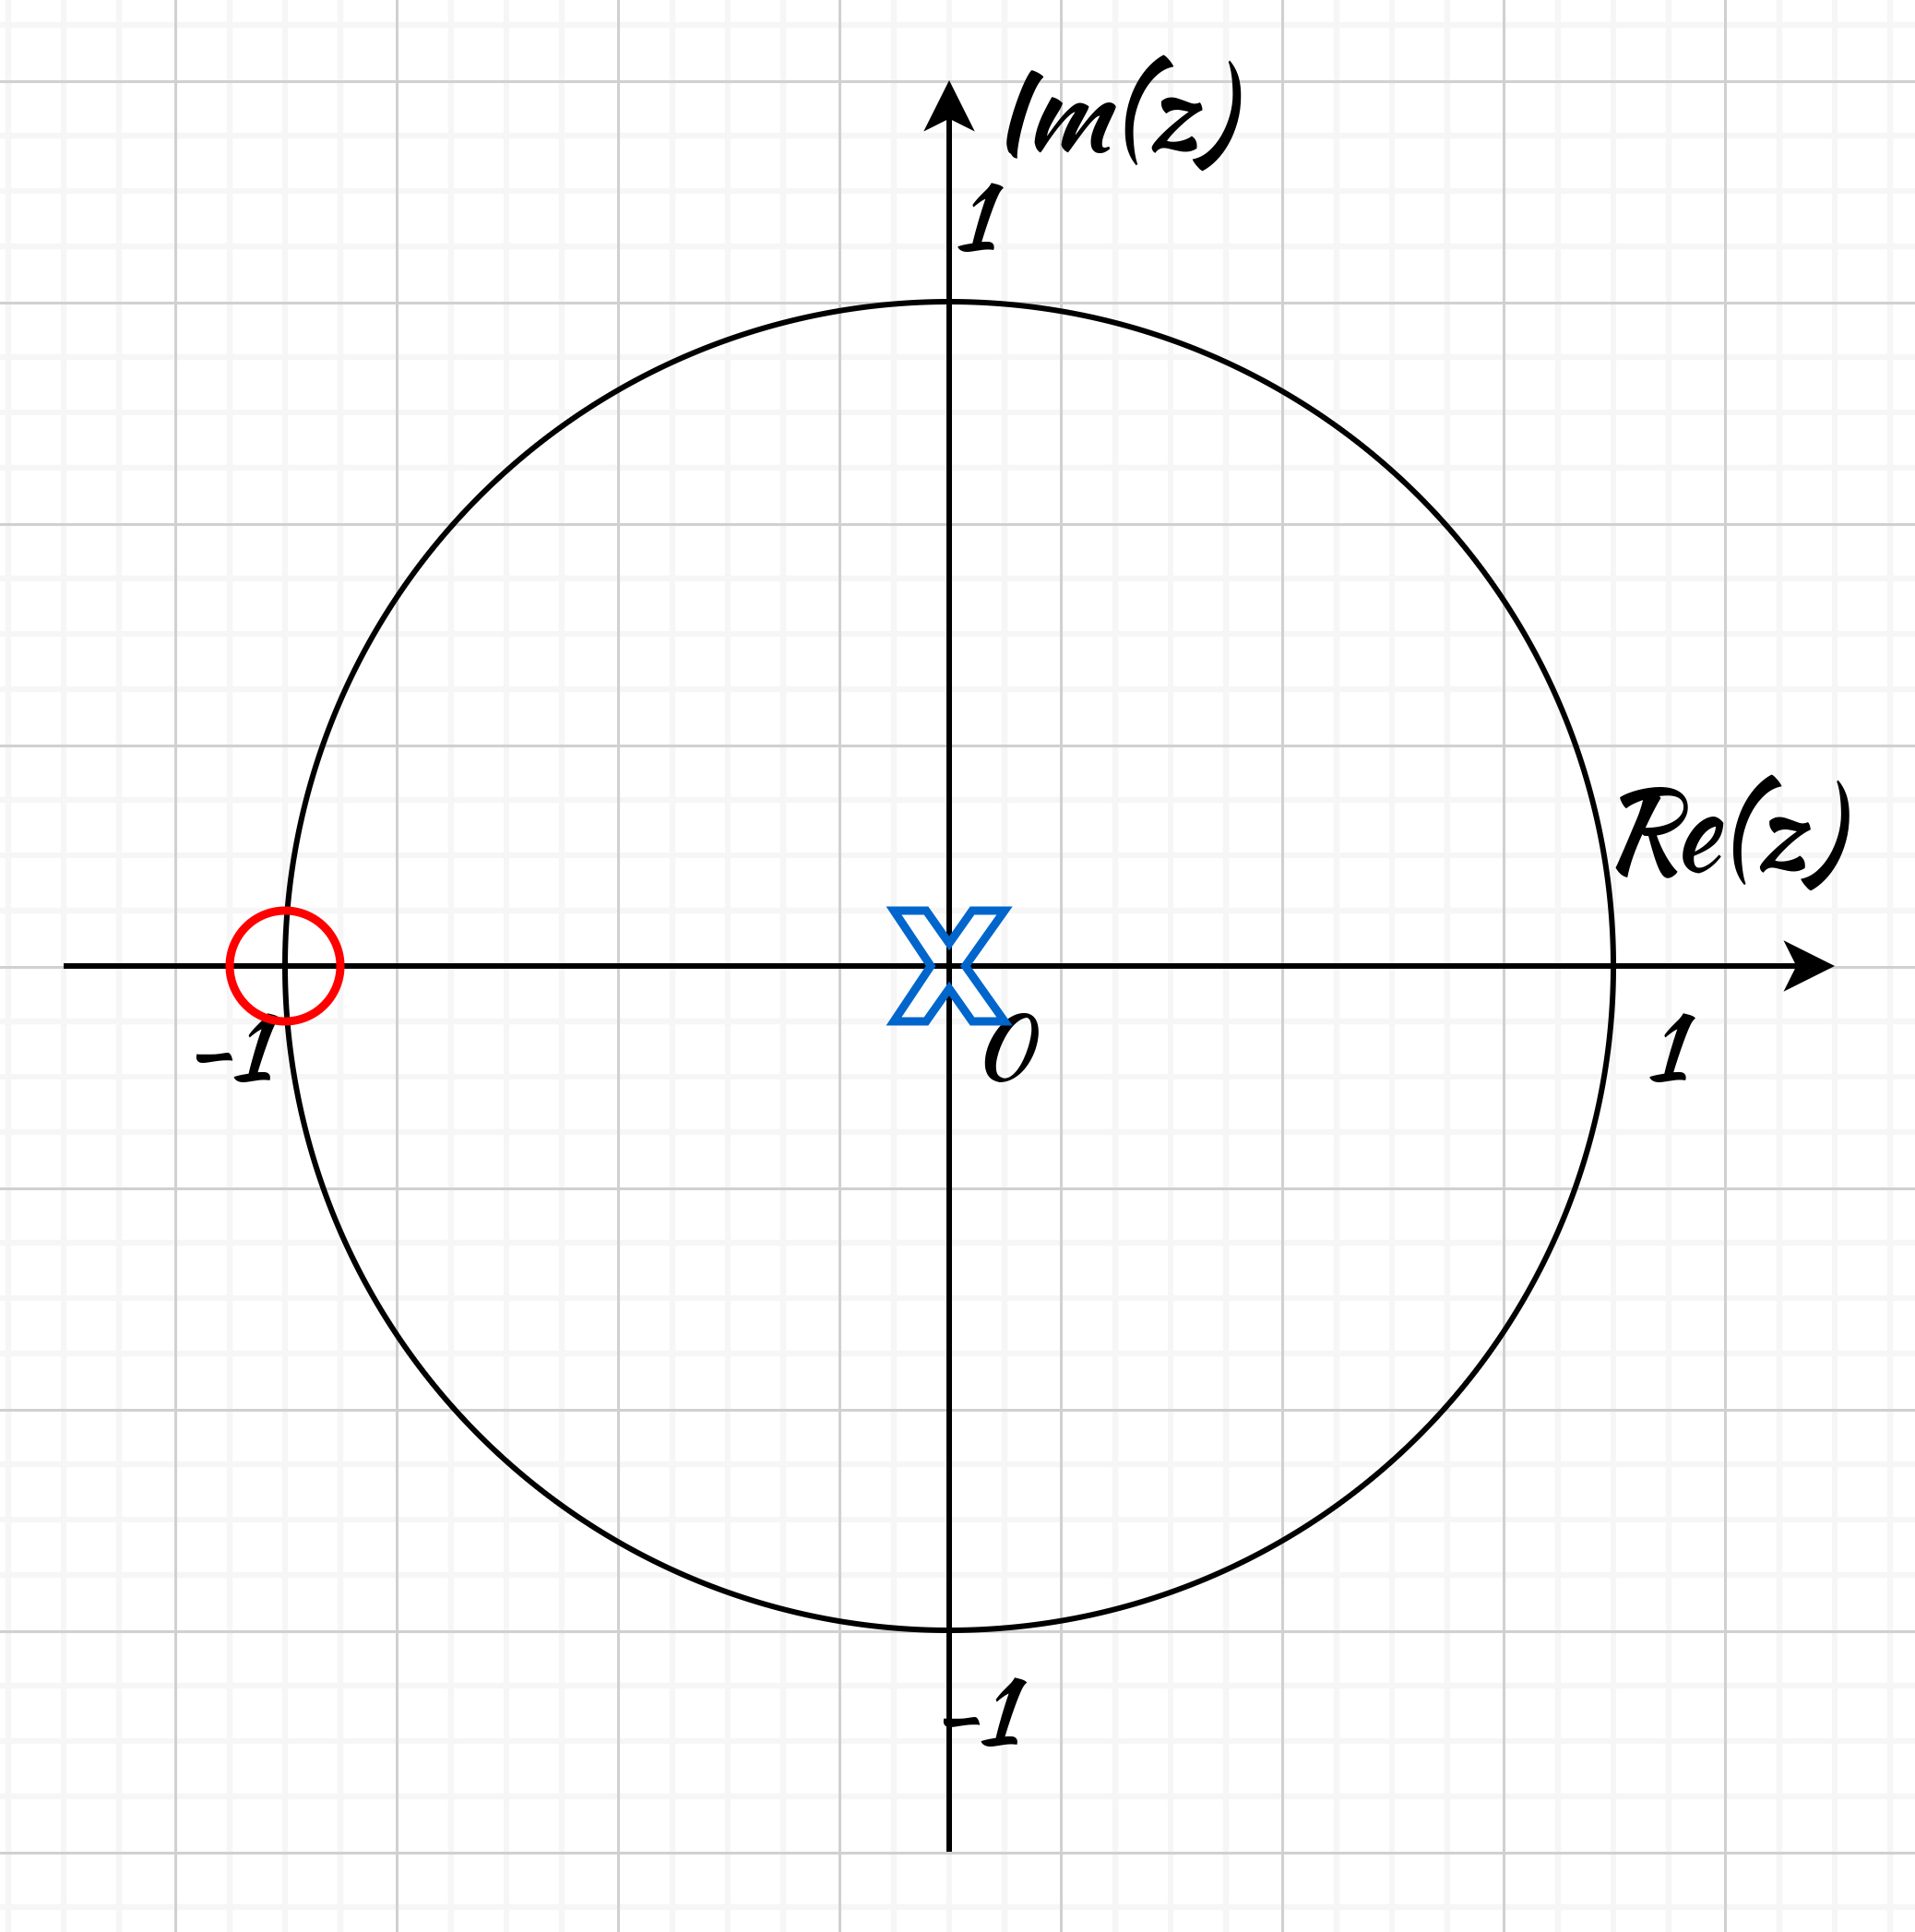
\includegraphics[width=0.4\columnwidth]{pics/fall/12/12-1-1.png}
	\label{fig:12-1-1}
\end{figure}

Единственный полюс $z_p = 0$ лежит внутри единичного круга на комплексной плоскости, то есть
система является устойчивой по входу.



\section{}
Для нерекурсивного фильтра второго порядка с передаточной функцией
\begin{equation*}
	\Capit{H}(z) = 1 - 0.1z^{-1} - 0.9z^{-2}
\end{equation*}
построить блок-схему реализации в прямой форме и в виде последовательного соединённых нерекурсивных фильтров первого порядка. Построить нуль-полюсную диаграмму и исследовать фильтр на устойчивость. Определить импульсную характеристику $h[k]$ и переходную характеристику $g[k]$ фильтра.

\begin{align*}
	\Capit{H}(z) = 1 - 0.1z^{-1} - 0.9z^{-2} = \Big(1 - z^{-1}\Big)\Big(1 + \frac{9}{10}z^{-1}\Big) =
	\dfrac{\Big(z - 1\Big)\Big(z + \dfrac{9}{10}\Big)}{z^2},\\
	z_{p} = 0,\; \s{k}_p = 2,\quad z_{o_1} = 1,\; z_{o_2} = -\dfrac{9}{10}.
\end{align*}

\begin{figure}[!h]
	\centering
	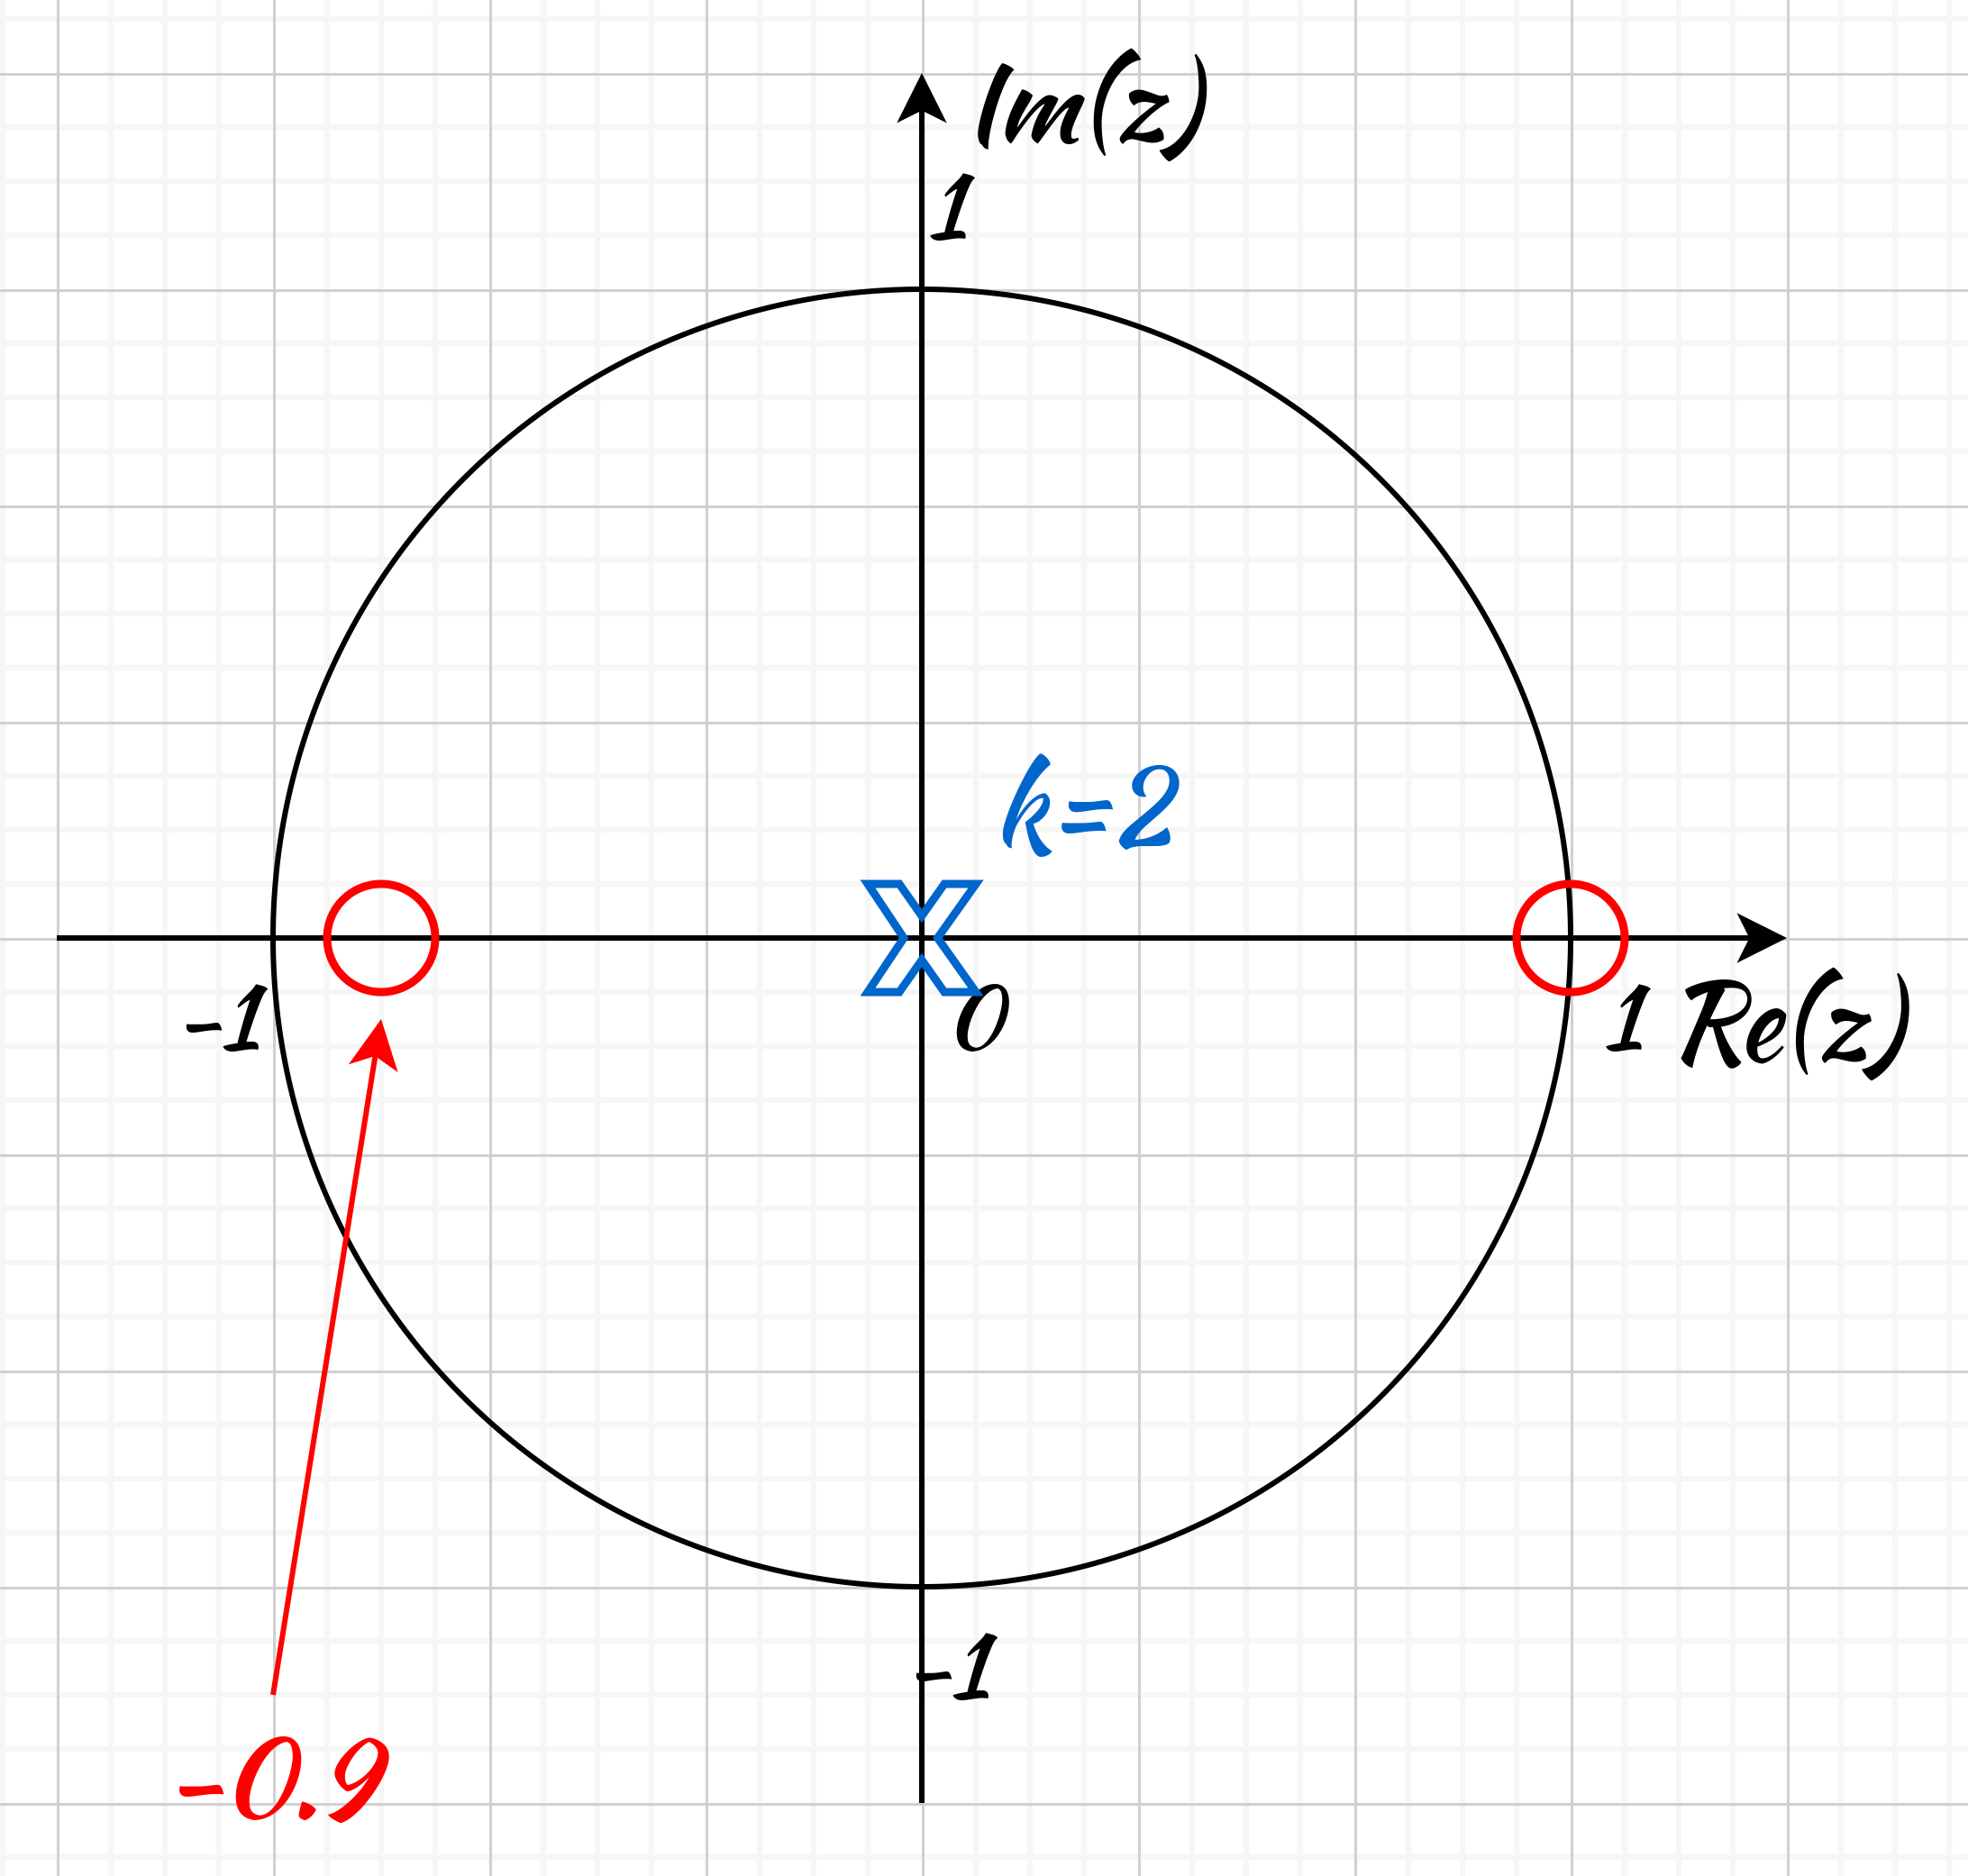
\includegraphics[width=0.4\columnwidth]{pics/fall/12/12-2-1.png}
	\label{fig:12-2-1}
\end{figure}


\begin{equation*}
	\Capit{H}(z) = 1 - 0.1z^{-1} - 0.9z^{-2} =  h[0] + h[1]z^{-1} + h[2]z^{-2},
	\quad \Rightarrow h[k] = 
	\begin{cases}
		1, & \text{если } k = 0,\\
		-0.1, & \text{если } k = 1,\\
		-0.9, & \text{если } k = 2,\\
		0, & \text{иначе}.
	\end{cases}
\end{equation*}

\begin{equation*}
	g[k] = \sum \limits_{m = 0}^{+\infty} h[k + m] = 
	\begin{cases}
		1, & \text{если } k = 0,\\
		0.9, & \text{если } k = 1,\\
		0, & \text{иначе}.
	\end{cases}
\end{equation*}


\begin{figure}[!h]
	\centering
	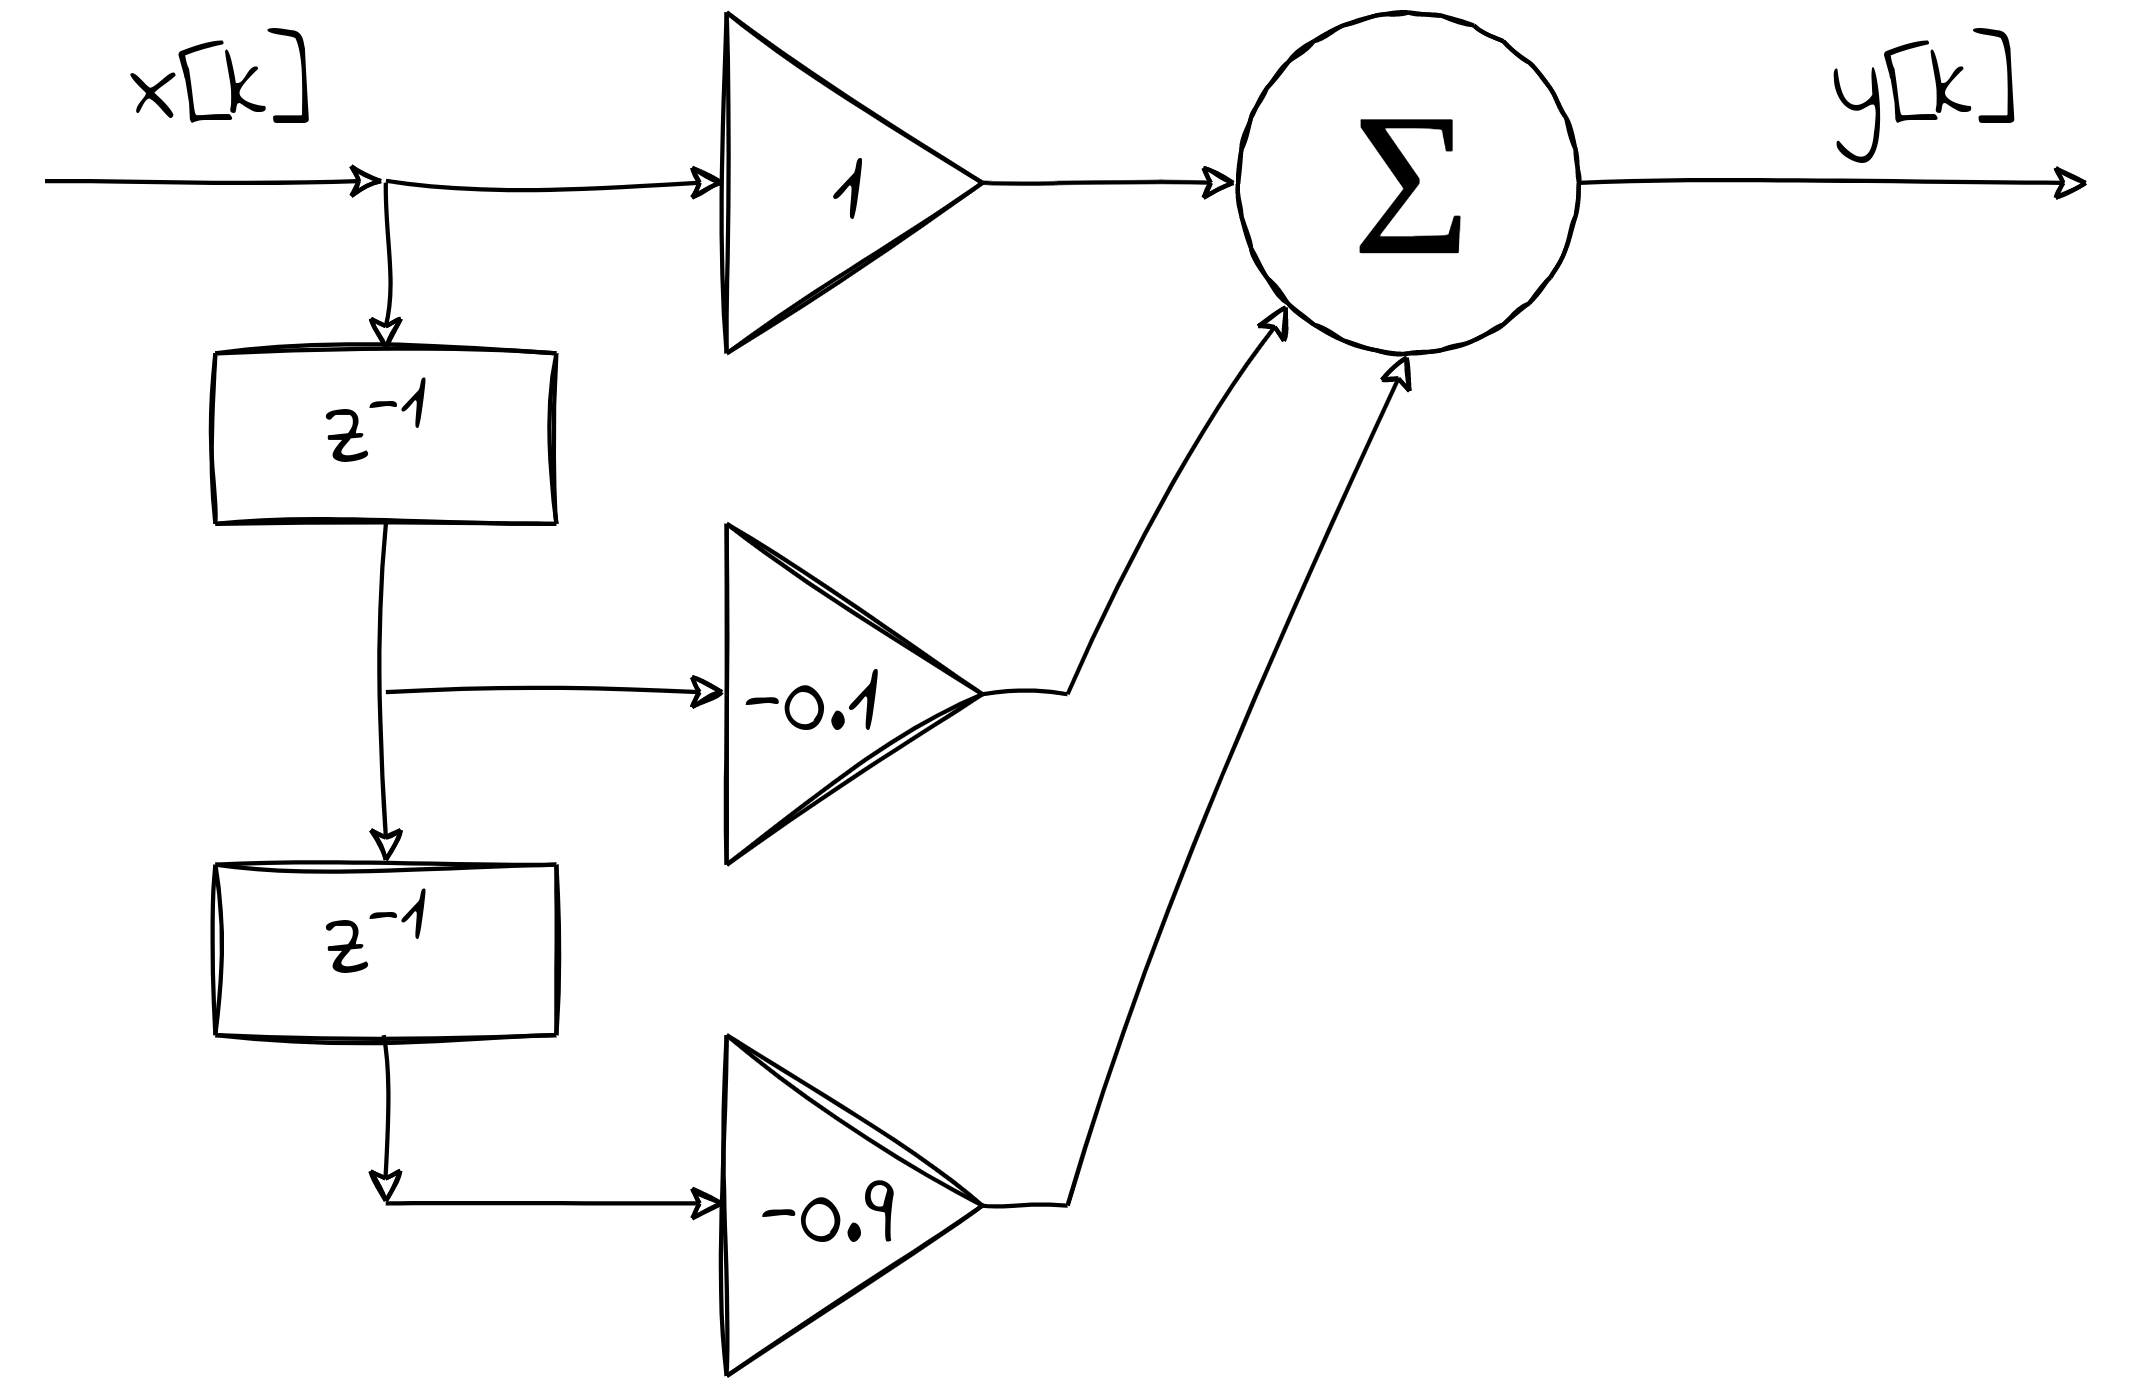
\includegraphics[width=0.75\columnwidth]{pics/fall/12/12-2-2.png}
	\caption{Блок-схема фильтра в прямой форме.}
	\label{fig:12-2-2}
\end{figure}

\begin{figure}[!h]
	\centering
	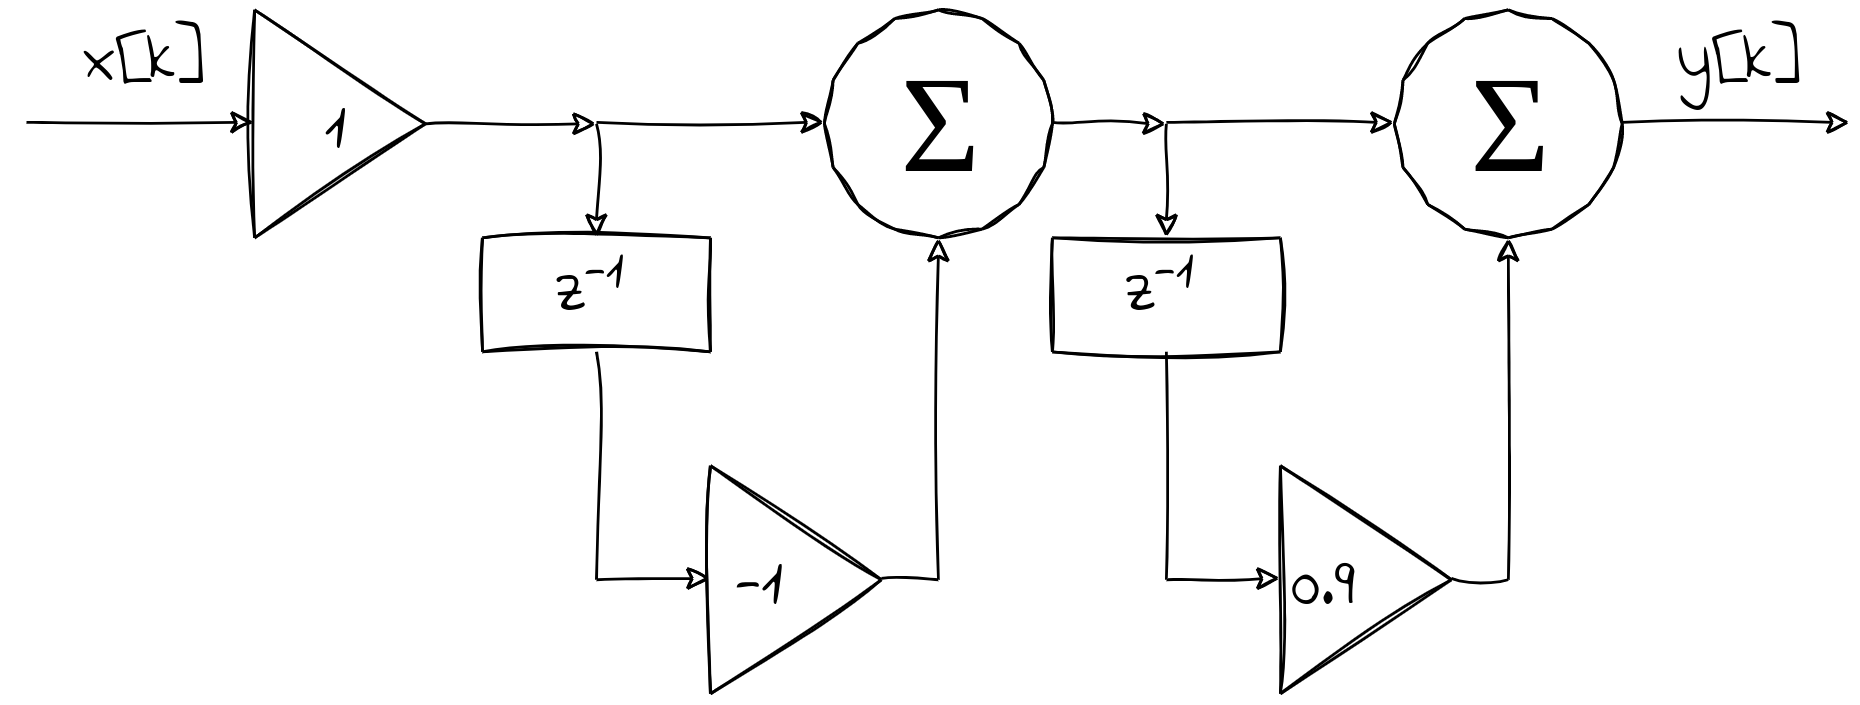
\includegraphics[width=0.75\columnwidth]{pics/fall/12/12-2-3.png}
	\caption{Блок-схема фильтра в виде последовательного соединённых нерекурсивных фильтров первого порядка.}
	\label{fig:12-2-3}
\end{figure}






\section{}
Записать разностное уравнение нерекурсивного фильтра второго порядка, передаточная функция которого содержит два комплексно-сопряженных нуля, расположенных на мнимой оси, а частотная характеристика фильтра $\Capit{H}(\theta)$ равна нулю в точках $\theta = \pm \frac{\pi}{2}$ и единице в точках $\theta = 0$ и $\theta = \pi$. Определить АЧХ и ФЧХ фильтра. Вычислить импульсную характеристику такого фильтра. Определить, будет ли ФЧХ такого фильтра линейной.

Определить, к какому классу частотно-избирательных фильтров его можно отнести:

\begin{enumerate}[label=(\alph*)]
	\item фильтры нижних частот,
	\item фильтры верхних частот,
	\item полосовые фильтры,
	\item режекторные фильтры.
\end{enumerate}

Передаточная функция имеет два комплексно-сопряженных нуля, расположенных на мнимой оси. Без ограничения общности, $z_o = j y$, $y \in \mathbb{R}$. Пусть $\s{k} \in \mathbb{R}$ -- множитель в приведённой форме $\Capit{H}(z)$.

\begin{equation*}
	\Capit{H}(z) = \s{k}(z - z_o)(z - z_o^*) = \s{k} (z - jy)(z + jy) = \s{k}(z^2 + y^2),
	\quad \Rightarrow \Capit{H}(\theta) = \Capit{H}(z)\big|_{z = e^{j \theta}} = \s{k}(e^{2j\theta} + y^2).
\end{equation*}

\begin{align*}
	&\Capit{H}(0) = \Capit{H}(\pi) =  \Capit{H}(\theta)\big|_{\theta = 0} = \s{k}(1 + y^2) = 1.\\
	&\Capit{H}(\pm \pi/2) =  \Capit{H}(\theta)\big|_{\theta = \pm \frac{\pi}{2}} = \s{k}(-1 + y^2) = 0.\\
	&\begin{cases}
		\s{k}(+1 + y^2) = 1\\
		\s{k}(-1 + y^2) = 0\\
	\end{cases} \Leftrightarrow
	\begin{cases}
		y = \pm 1\\
		\s{k} = 0.5\\
	\end{cases}
\end{align*}

\begin{align*}
	&\Capit{H}(\theta) = 0.5(1 + e^{2j\theta}) = 0.5 e^{-j\theta} (e^{j\theta} + e^{-j\theta}) = e^{-j\theta} \cos\theta.\\
	&|\Capit{H}(\theta)| = |\cos\theta|,\quad
	\arg\{\Capit{H}(\theta)\} = \arg\{e^{-j\theta}\} = -\theta, \; \Rightarrow \text{ ФЧХ линейная}.
\end{align*}

Этот фильтр относится к гребенчатым фильтрам, поскольку его АЧХ имеет гребенчатую структуру.
Если же рассматривать главный период, то его можно отнести к режекторным фильтрам.
